\documentclass[11pt]{article}
\usepackage[utf8]{inputenc} 
\usepackage[T1]{fontenc}    
\usepackage{url}            
\usepackage{booktabs}       
\usepackage{amsfonts}       
\usepackage{nicefrac}
\usepackage{microtype}      
\usepackage{fullpage}
\usepackage{subcaption}
\usepackage[most]{tcolorbox}
\usepackage[numbers]{natbib}
%\usepackage[textsize=tiny]{todonotes}
\setlength{\marginparwidth}{11ex}

\newcommand{\E}{\mathbb E}
\usepackage{wrapfig}
\usepackage{caption}

\newcommand{\theHalgorithm}{\arabic{algorithm}}

\usepackage{url}

\usepackage[utf8]{inputenc}
\usepackage{amsmath}
\usepackage{graphicx}
\usepackage{upgreek}
\usepackage{amsfonts}
\usepackage{amssymb}
\usepackage{amsthm}
\usepackage[mathscr]{euscript}
\usepackage{mathtools}
\newtheorem{thm}{Theorem}
\newtheorem{defn}{Definition}
\newtheorem{cor}{Corollary}
\newtheorem{assumption}{Assumption}
\newtheorem{lem}{Lemma}
\usepackage{xcolor}
\usepackage{nicefrac}
\usepackage{xr}
%\usepackage{chngcntr}
\usepackage{apptools}
\usepackage[page, header]{appendix}
\AtAppendix{\counterwithin{lem}{section}}
\usepackage{titletoc}
\usepackage{enumitem}
\setlist[itemize]{leftmargin=1cm}
\setlist[enumerate]{leftmargin=1cm}
\newcommand*{\fnref}[1]{\textsuperscript{\ref{#1}}}



\definecolor{DarkRed}{rgb}{0.75,0,0}
\definecolor{DarkGreen}{rgb}{0,0.5,0}
\definecolor{DarkPurple}{rgb}{0.5,0,0.5}
\definecolor{Dark}{rgb}{0.5,0.5,0}
\definecolor{DarkBlue}{rgb}{0,0,0.7}
\usepackage[bookmarks, colorlinks=true, plainpages = false, citecolor = DarkBlue, urlcolor = blue, filecolor = black, linkcolor =DarkGreen]{hyperref}
\usepackage{breakurl}
\usepackage[ruled, vlined, linesnumbered]{algorithm2e}
\newcommand\mycommfont[1]{\footnotesize\ttfamily\textcolor{blue}{#1}}
\SetCommentSty{mycommfont}

\DeclareMathOperator*{\argmin}{arg\,min}
\DeclareMathOperator*{\argmax}{arg\,max}

\allowdisplaybreaks[2]
\newcommand{\prob}{\mathbb P}
\newcommand{\Var}{\mathbb V}
\newcommand{\NN}{\mathbb N}
\newcommand{\Ex}{\mathbb E}
\newcommand{\varV}{\mathscr V}
\newcommand{\indicator}[1]{\mathbb I\{ #1 \} }
\newcommand{\statespace}{\mathcal S}
\newcommand{\actionspace}{\mathcal A}
\newcommand{\saspace}{\statespace \times \actionspace}
\newcommand{\satspace}{\mathcal Z}
\newcommand{\numsa}{\left|\saspace\right|}
\newcommand{\numsat}{\left|\satspace\right|}
\newcommand{\numS}{S}
\newcommand{\numA}{A}
\newcommand{\wmin}{w_{\min}}
\newcommand{\wminc}{w'_{\min}}
\newcommand{\range}{\operatorname{rng}}
\newcommand{\polylog}{\operatorname{polylog}}
\newcommand{\dspace}{\mathcal D}
\newcommand{\numD}{|\dspace|}
\newcommand{\numSucc}[1]{|\statespace(#1)|}
\newcommand{\succS}[1]{\statespace(#1)}

\newcommand{\reals}{\mathbb R}
\newcommand{\const}{\textrm{const.}}
\newcommand{\set}[1]{\left\{#1\right\}}
\newcommand{\llnp}{\operatorname{llnp}}
\newcommand{\defeq}{:=}
\usepackage{xspace}
\newcommand{\algname}{UBEV\xspace}

\mathtoolsset{showonlyrefs=true}

\let\temp\epsilon
\let\epsilon\varepsilon
\newcommand{\cK}{\mathcal K}
\newcommand{\cI}{\mathcal I}
\newcommand{\Pro}{\mathbb P}

\title{CS 234 Winter 2022 \\ Assignment 1 \\ Due: January 14 at 6:00 pm (PST)}
\date{}

\begin{document}
  \maketitle
\noindent For submission instructions, please refer to \href{http://web.stanford.edu/class/cs234/assignments.html}{website}.
For all problems, if you use an existing result from either the literature or a textbook to solve the exercise, you need to cite the source.


\section{Efficient Routing MDP [35 pts]}

You are leading a routing and planning team at a self-driving car company and have decided to model your latest urban navigation problem as an MDP. Consider the following environment (Fig. \ref{fig:fig1}). Your car must navigate along the road (gray squares) while avoiding obstacles (red squares) to reach the rider's destination (the green square). Because the road is gridlocked, your car must change lanes whenever it wishes to move forward. From any gray square, your car can either move right $\&$ up, or  right $\&$ down. For example, starting from state $3$, your car can move to state $8$ or $10$. Note that it is not be possible to reach the green square from every state. Actions are deterministic and always succeed unless they will cause you to run into an impassible barrier. The thick outer edge indicates an impassible barrier, and attempting to move in the direction of a barrier from a gray square results in your car moving up one square (e.g. taking any action from state 32 moves the car to state 31). 

\begin{figure}[ht]
\begin{subfigure}{.5\textwidth}
  \centering
  % include first image
  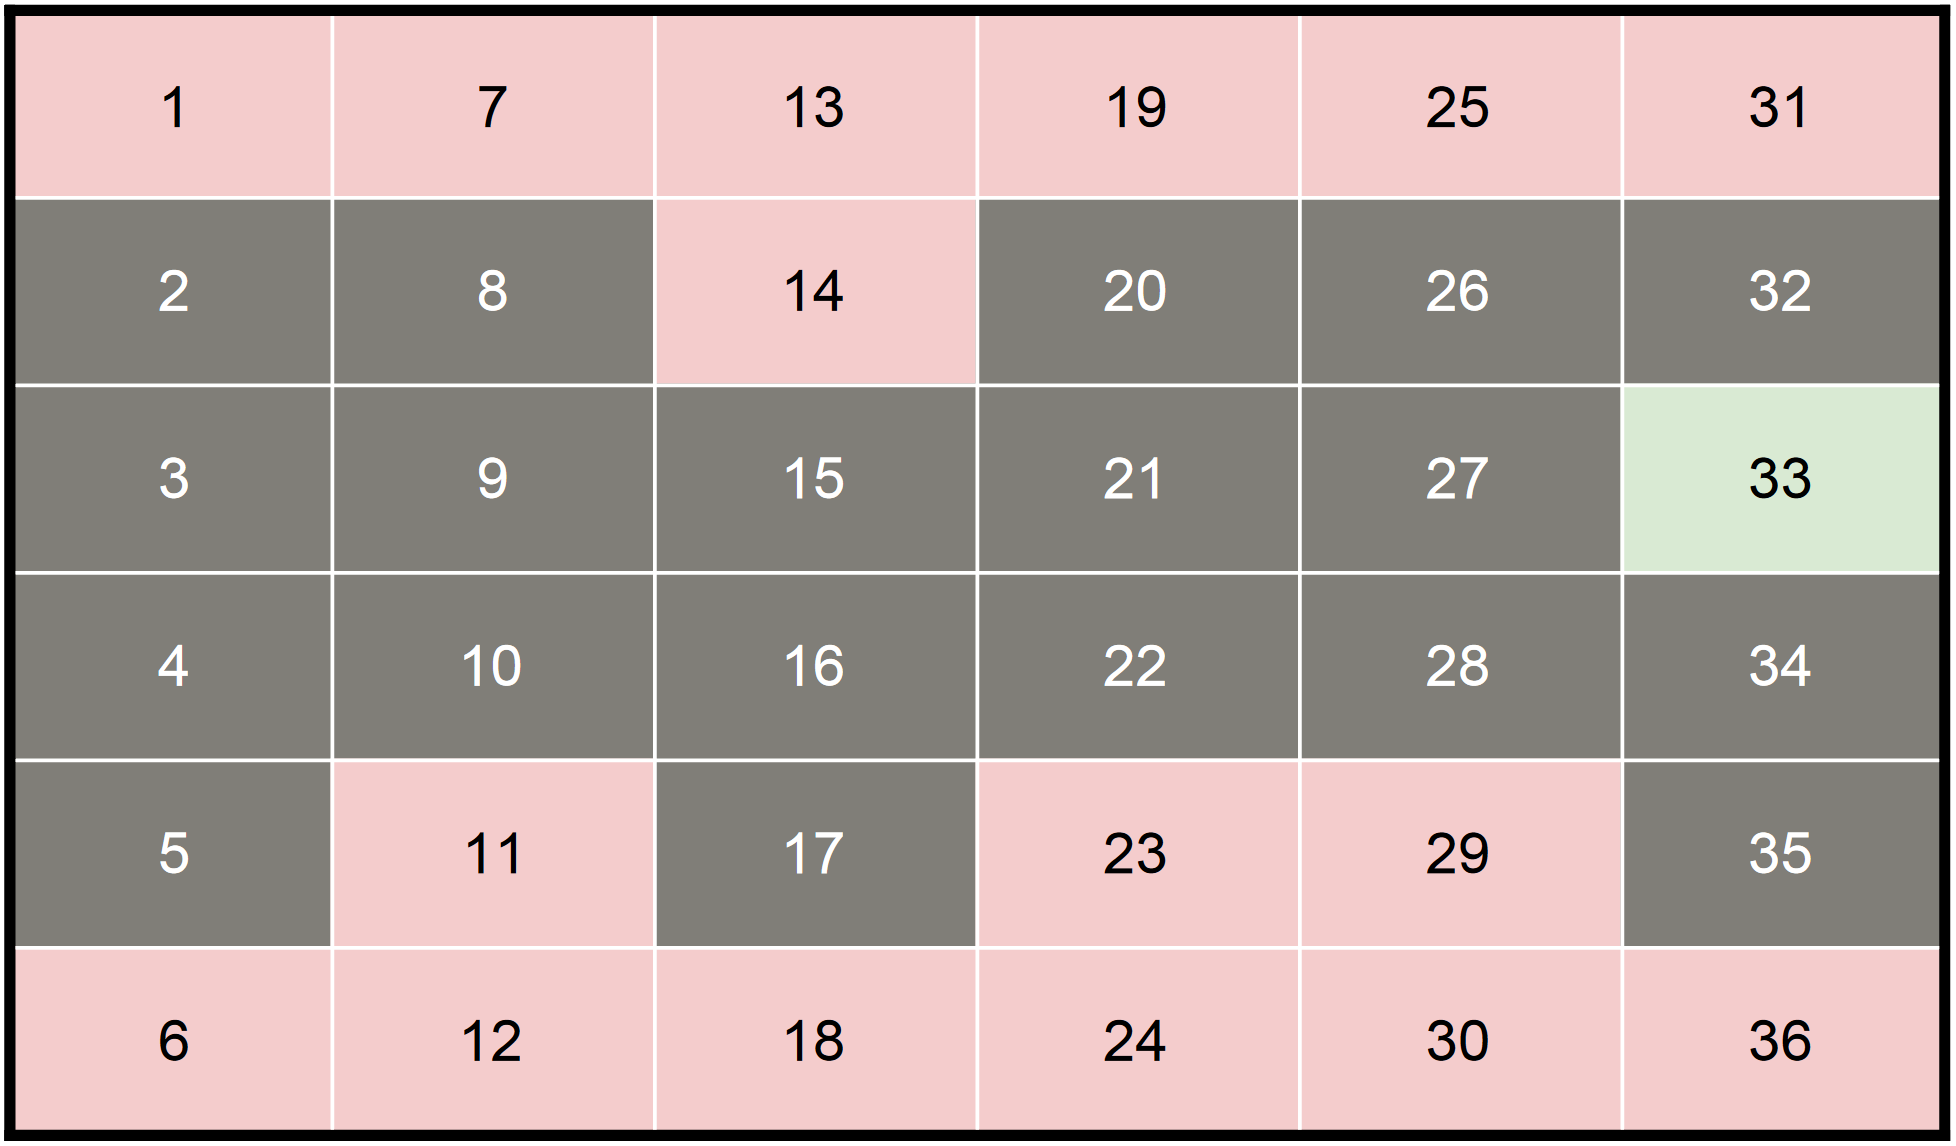
\includegraphics[width=.9\linewidth]{gridworld.png}  
  \caption{Grid World}
  \label{fig:fig1.a}
\end{subfigure}
\begin{subfigure}{.5\textwidth}
  \centering
  % include second image
  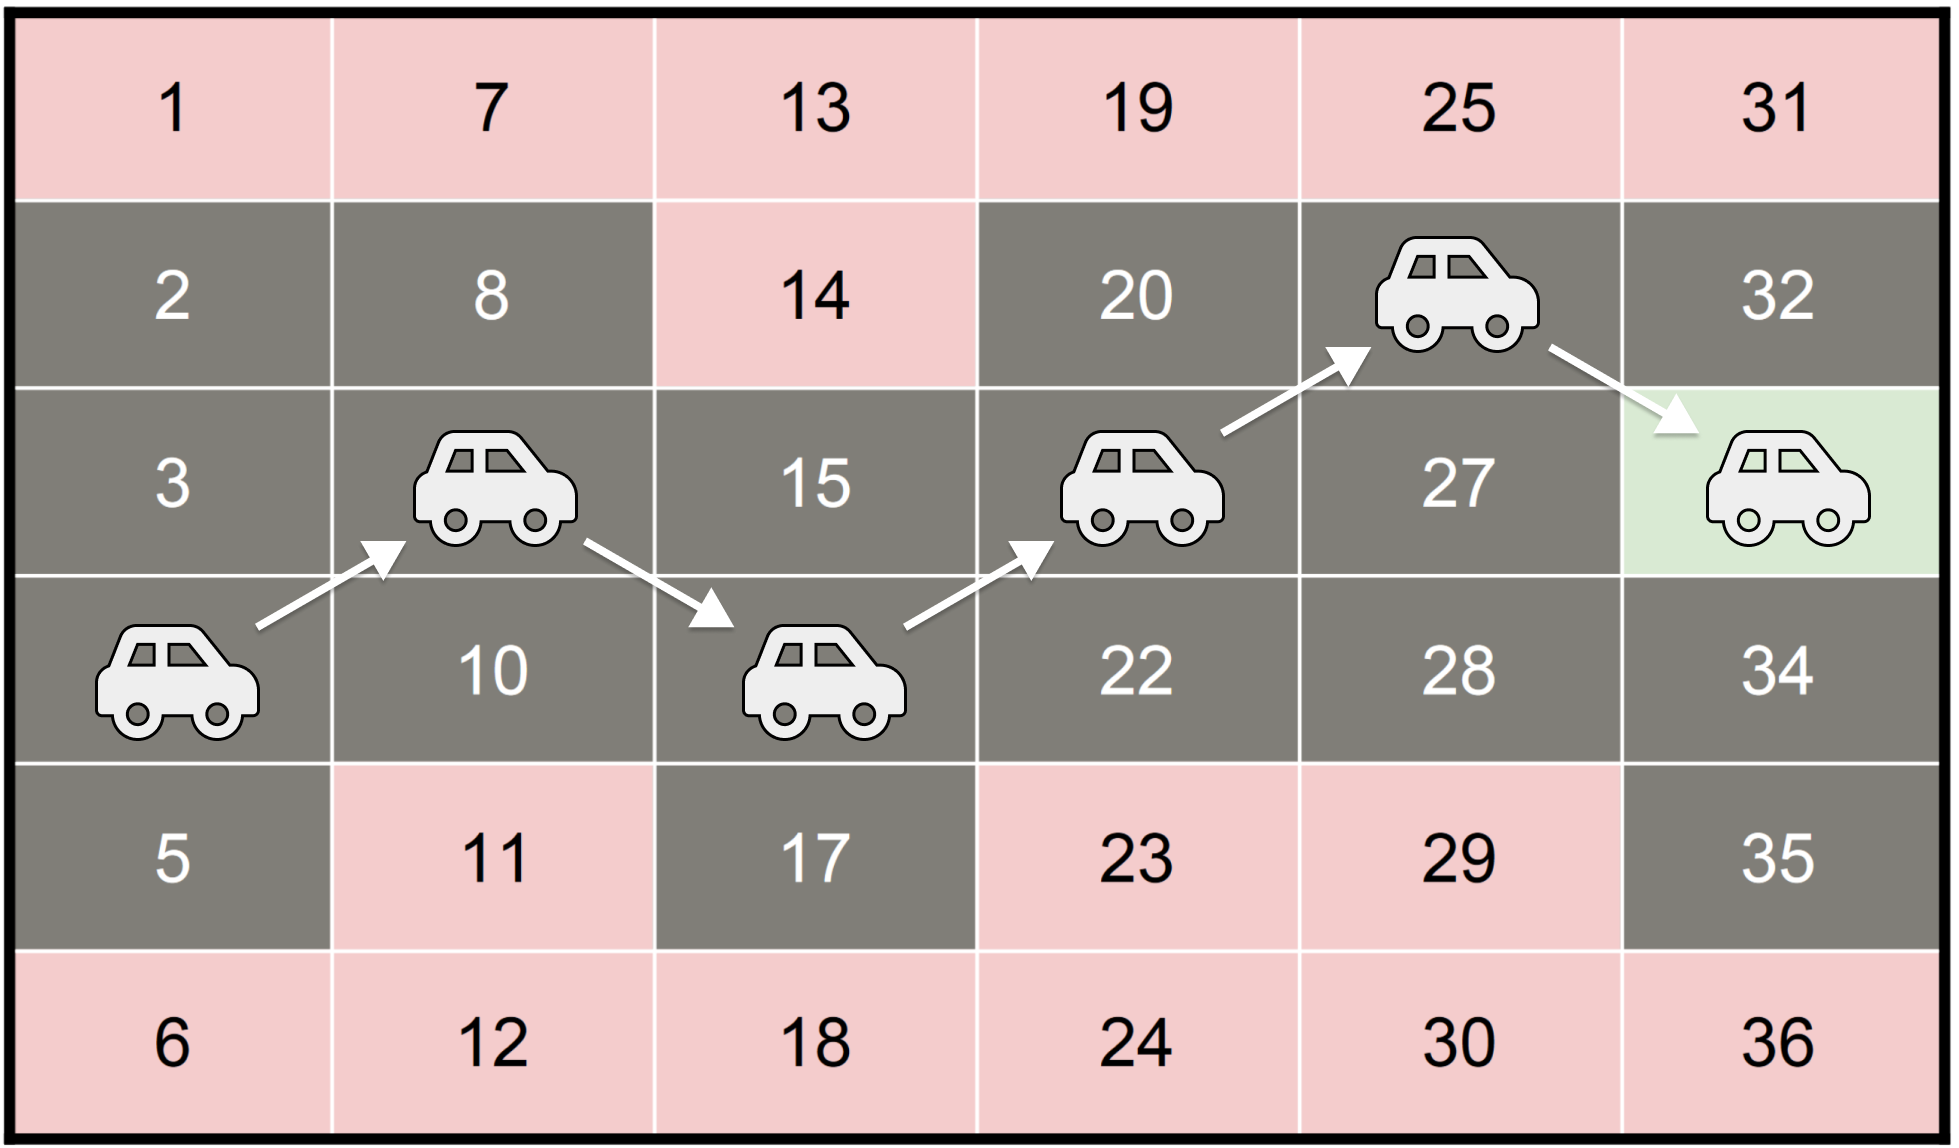
\includegraphics[width=.9\linewidth]{gridworldcar2.png}  
  \caption{A successful run in Grid World.}
  \label{fig:fig1.b}
\end{subfigure}
\caption{}
\label{fig:fig1}
\end{figure}

A successful run in Grid World 1 is shown in Figure \ref{fig:fig1.b}. Taking any action from the green destination square (no. 33) earns a reward of $r_g$  and ends the episode. Taking any action from the red squares that depict obstacles (no. 1, 7, 13...) earns a reward of $r_r$ and ends the episode. Otherwise, from every other square, taking any action is associated with a reward $r_s$. Assume the discount factor $\gamma = 0.9$, $r_g = +5$, and $r_r = -5$ unless otherwise specified. Notice the horizon is technically infinite. 

\begin{enumerate}[label=(\alph*)]
\item  Let $r_s \in \{-5,-0.5,0,2\}$. Starting in \textbf{square 2}, for each of the possible values of $r_s$, briefly explain what the optimal policy would be in Grid World. In each case is the optimal policy unique and does the optimal policy depend on the value of the discount factor $\gamma$? Explain your answer.   [5 pts]


\item Which values of $r_s \in \{-5, -0.5, 0, 2\}$ will yield a policy that returns the shortest path to the green square? (Hint: At least one does.) Explain which ones do, then, pick the minimum of this set of rewards that does, and then find the optimal value function for \textbf{states 2, 13, 21 and 32}. [5 pts]

\end{enumerate}

\noindent Rather than finding the shortest path between two points, suppose our car is low on gas, so we want to take the path that uses the least fuel. In the real world, navigation optimized for fuel consumption may take more steps to reach a destination \footnote{\href{https://blog.google/products/maps/3-new-ways-navigate-more-sustainably-maps/}{Google Maps Blog}}. 

Consider the same MDP, but with two new ``efficient actions'' -- move right or move down. For example, starting from state 3, you can either move to state 4 or 9. Once again, the actions are deterministic and always succeed unless you run into a wall. Attempting to move in the direction of a wall from a gray square using an efficient action results in you moving \textit{down} one square. For clarity, we will use separate symbols $r_s$ for the reward associated with an inefficient action (right $\&$ up, or  right $\&$ down) and $r_e$ for the reward associated with an efficient action.

\begin{enumerate}

\item[(c)] Let $r_e \in \{-5,-0.5,0,2\}$. Starting in \textbf{state 2}, for each of the possible values of $r_e$, briefly explain what the optimal policy would be in Grid World \textit{using only efficient actions}. In each case is the optimal policy unique and does the optimal policy depend on the value of the discount factor $\gamma$? Explain your answer. Which values of $r_e$ would cause the optimal policy to return the shortest path to the green destination square?  [5 pts]

\item[(d)] Consider now that $r_s = 0$. Derive a relation for $r_e$ such that the optimal path from \textbf{state 2} to the destination square using only efficient actions is strictly more rewarding than the optimal path using only inefficient actions.  [5 pts]

\item[(e)] Compare the set of gray states that can reach the goal using only efficient actions, and the set of gray states that can reach the goal using only inefficient actions. Which states are part of one set but not part of the other? Explain your answer. [5 pts]

\item [(f)] Consider a general MDP with rewards and transitions. Consider a discount factor of $\gamma$. Assume that the horizon is infinite (so there is no termination). Can adding a constant c to all rewards ($r_{new} = c + r_{old}$) change the optimal policy of the MDP? If yes, give an example for Grid World with efficient actions using the $r_g$, $r_s$ and $r_e$ such that the optimal policy changes for a specific constant. [5 pts]

\item[(g)]
Imagine your efficient routing MDP is to be used in a popular maps app or website.  Choosing what route options will be available and which will be default present inevitable value judgements. The shortest path and the sustainable path are each optimal given their choices of rewards, but the rewards formalize different values.  How would you present the shortest path and sustainable path options in a maps app and why? Please use 2-4 sentences to explain your answer. There is no single ``correct'' answer-- reasonable explanations of your choice will receive full credit. [5 pts]

Context for the debate: “Green nudges” such as setting the most efficient route as the (changeable) default on mapping apps have been proposed as a way to encourage environmentally beneficial actions.\footnote{A nudge is an “aspect of  choice architecture that alters people’s behaviour in a predictable way without forbidding any options or significantly changing economic incentives” (\href{https://psycnet.apa.org/record/2008-03730-000}{Thaler and Sunstein, 2008}).}  They can help close the gap between the desire to act more sustainably that many people express and their day to day behavior.\footnote{\label{note2}Siipi and Koi, 2021. https://philpapers.org/archive/SIITEO.pdf}  Some have argued that green nudges do not go far enough and that given the urgency of climate change the sustainable option should be the only one presented. Others argue that nudges infringe autonomy and so users should be explicitly asked which default they would prefer; others that nudges are only acceptable when the intention behind the nudge is transparently presented. For more context, see [\ref{note2}].
\end{enumerate}

\begin{tcolorbox}[breakable]
  
\end{tcolorbox}

\newpage

\section{Value Iteration Theorem [35 pts]}



In this problem, we will deal with contractions and fixed points and prove an important result from the value iteration theorem.
From lecture, we know that the Bellman backup operator $B$ given below is a contraction with the fixed point as $V^*$, the optimal value function of the MDP. The symbols have their usual meanings. $\gamma$ is the discount factor and $0 \leq \gamma < 1$. In all parts, $||v||$ is the infinity norm of the vector.
\begin{equation}
    (BV)(s) = \max_a[ R(s, a) + \gamma\sum_{s' \in S}p(s'|s,a)V(s')]
\end{equation}

We also saw the contraction operator $B_\pi$ which is the Bellman backup operator for a particular policy given below:
\begin{equation}
    (B_\pi V)(s) =  \E_{a \sim \pi}[R(s,a) + \gamma\sum_{s' \in S}p(s'|s,a)V(s')]
\end{equation}

\begin{enumerate}[label=(\alph*)]
    \item Recall that $||BV - BV'|| \leq \gamma ||V - V'||$ for two random value functions $V$ and $V'$. Prove that $B_\pi$ is also a contraction mapping:  $||B_\pi V - B_\pi V'|| \leq \gamma ||V - V'||$. [5 pts]
    \item Prove that the fixed point for $B_\pi$ is unique. What is the fixed point of $B_\pi$? [5 pts]
\end{enumerate}

\noindent In value iteration, we repeatedly apply the Bellman backup operator $B$ to improve our value function. At the end of value iteration, we can recover a greedy policy $\pi$ from the value function using the equation below:

\begin{equation}
    \pi(s) = \argmax_{a} [{r(s,a) + \gamma\sum_{s' \in S}p(s'|s,a)V(s')}]
\end{equation}

\noindent Suppose we run value iteration for a finite number of steps to obtain a value function $V$ ($V$ has not necessarily converged to $V^*$). Say now that we evaluate our policy $\pi$ obtained using the formula above to get $V^\pi$. \textbf{Note that here and for the rest of Q2, $\pi$ refers to the greedy policy.}

\begin{enumerate}
    \item[(c)] Is $V^{\pi}$ always the same as $V$? Justify your answer. [5 pts]
\end{enumerate}

\noindent In lecture, we learned that running value iteration until a certain tolerance can bring us close to recovering the optimal value function. Let $V_{n}$ and $V_{n+1}$ be the outputs of value iteration at the $n^{th}$ and $n+1^{th}$ iterations respectively. Let  $\epsilon > 0$ and consider the point in value iteration such that $||V_{n+1} - V_{n}|| < \frac{\epsilon (1 - \gamma)}{2\gamma}$. Let $\pi$ be the greedy policy given the value function $V_{n+1}$. 

\noindent You will now prove that this policy $\pi$ is $\epsilon$-optimal. This result justifies why halting value iteration when the difference between success iterations is sufficiently small, ensures the decision policy obtained by being greedy with respect to the value function, is near-optimal. 

\noindent Precisely if 
\begin{equation}
    ||V_{n+1} - V_{n}|| < \frac{\epsilon (1 - \gamma)}{2\gamma}
\end{equation}
then, 
\begin{equation}
    ||V^{\pi} - V^{*}|| \leq \epsilon
\end{equation}


\begin{enumerate}
    \item[(d)] When $\pi$ is the greedy policy, what is the relationship between $B$ and $B_\pi$? [2 pts]
    \item[(e)] Prove that $||V^{\pi} - V_{n+1}|| \leq \epsilon /2$. \\ 
    \textbf{Hint: }Introduce an in-between term and leverage the triangle inequality. [6 pts]
    \item[(f)] Prove  $||B^kV - B^kV'|| \leq \gamma^k||V - V'||$ [3 pts]
    \item[(g)] Prove that $||V^{*} - V_{n+1}|| \leq \epsilon /2$. [7pts]\\ 
    \textbf{Hints: } Note that $||V^{*} - V_{n+1}|| = ||V^{*} + V_{n+2} - V_{n+2} - V_{n+1}||$ and you can repeatedly apply this trick. It may also be useful to leverage part (f) and recall that $V^{*}$ is the fixed point of the contraction $B$. \\
\item[(h)] Use the results from parts (e) and (g), to show that $||V^{\pi} - V^{*}|| \leq \epsilon$ [2 pts]
\end{enumerate}


\begin{tcolorbox}[breakable]
\end{tcolorbox}


\newpage

\begin{section}{Frozen Lake MDP [25 pts]}
Now you will implement value iteration and policy iteration for the Frozen Lake environment
from \href{"https://gym.openai.com/envs/FrozenLake-v0"}{OpenAI Gym}. We have provided
custom versions of this environment in the starter code.
\begin{enumerate}[label=(\alph*)]
\item \textbf{(coding)} Read through \texttt{vi\_and\_pi.py} and implement \texttt{policy\_evaluation}, \texttt{policy\_improvement} and \texttt{policy\_iteration}. The stopping tolerance (defined as $\max_s |V_{old}(s) - V_{new}(s)|$) is tol = $10^{-3}$
. Use $\gamma = 0.9$. Return the optimal value function and the optimal policy. [10pts]
\item \textbf{(coding)} Implement \texttt{value\_iteration} in \texttt{vi\_and\_pi.py}. The stopping tolerance is tol =
$10^{-3}$
. Use $\gamma = 0.9$. Return the optimal value function and the optimal policy. [10 pts]
\item \textbf{(written)} Run both methods on the Deterministic-4x4-FrozenLake-v0 and

Stochastic-4x4-FrozenLake-v0 environments. In the second environment, the dynamics of the world are stochastic. How does stochasticity affect the number of iterations required, and the resulting policy? [5 pts]

\end{enumerate}
\end{section}


\begin{tcolorbox}[breakable]
\end{tcolorbox}



\end{document} 